\section{Background to the Research}
\vspace{12pt}

According to the intellectual property act of Sri Lanka\cite{CopyrightAct}, royalties must be paid to the original
artistes when a song is broadcast on a radio channel. Each radio channel is maintaining a playlist to keep track of
the songs that were broadcast throughout the day. That playlist can later be used to pay royalties to the respective
artistes. However, in order to streamline and regulate the royalty payment process, it is vital to have a method to monitor the radio 
broadcasts. Manual radio broadcast monitoring is infeasible and expensive due to increasing number of both radio 
channels and songs. In manual monitoring a person should be assigned to each channel who needs to keep record of each 
song in the radio broadcast of that assigned channel. Due to the increasing number of songs and the fallible nature of
humans such a monitoring task is prone to errors and inaccuracies. Hence an automated radio broadcast 
monitoring approach must be considered as an viable alternative in the modern day radio broadcast monitoring.
\vspace{12pt}

\begin{figure}[H]
    \centering
    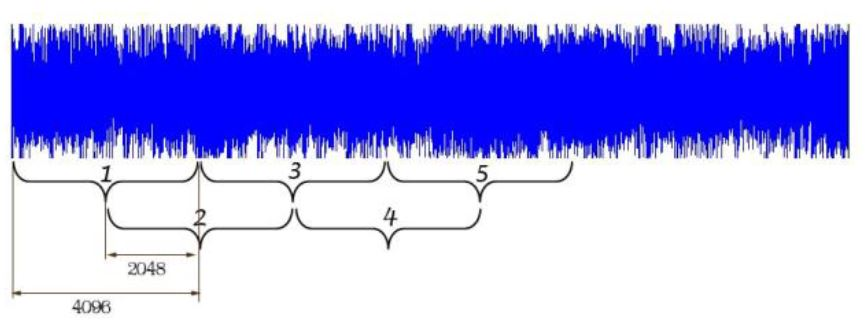
\includegraphics[scale=0.7]{STFT}
    \caption{Key controlling parameters of STFT\cite{Nishan}}
    \label{fig:stft}
\end{figure}
\vspace{12pt}

In the research \say{Radio Broadcast Monitoring to Ensure Copyright Ownership}\cite{Nishan}, researchers have implemented an
automated radio broadcast monitoring system (refer the Figure \ref{fig:existing_system} for the architecture) which has 
achieved 97.14\% overall accuracy in identifying original songs
in radio broadcasts. The researchers introduced an audio fingerprint to register and identify songs. The fingerprint was
introduced as a series of hash values extracted from frequency domain audio signal. Time domain signal was converted to 
frequency domain by using \ac{stft}, which used 4096 bits long window and 2048
bits long overlapping area as shown in Figure \ref{fig:stft}. Then five peak values were extracted for each window by 
dividing mid frequency level into five bins and taking peak value from each bin. Extracted five peak values were used to 
create a hash value as depicted in Figure \ref{fig:fingerprint}. 

\vspace{12pt}

\begin{figure}[H]
    \centering
    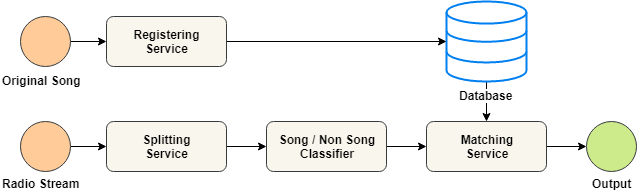
\includegraphics[scale=0.6]{ExistingSystem.png}
    \caption{Architecture of the existing system}
    \label{fig:existing_system}
\end{figure}
\vspace{12pt}

In contemporary radio broadcasts, channels tends to alter songs by including commercials and dialogues and by remastering 
the original song. Remastering can be done by adding or subtracting elements, or by changing pitch, equalization, dynamics or 
tempo\cite{SerraBook}. Even though the above mentioned radio broadcast monitoring system's accuracy is not significantly 
affected by commercials and dialogues included in songs, the system is unable to identify a song when that song is remastered 
by the radio channel as changing pitch, equalization, dynamics or tempo which directly affects both time domain and 
frequency domain audio data.

\vspace{12pt}

\begin{figure}[H]
    \centering
    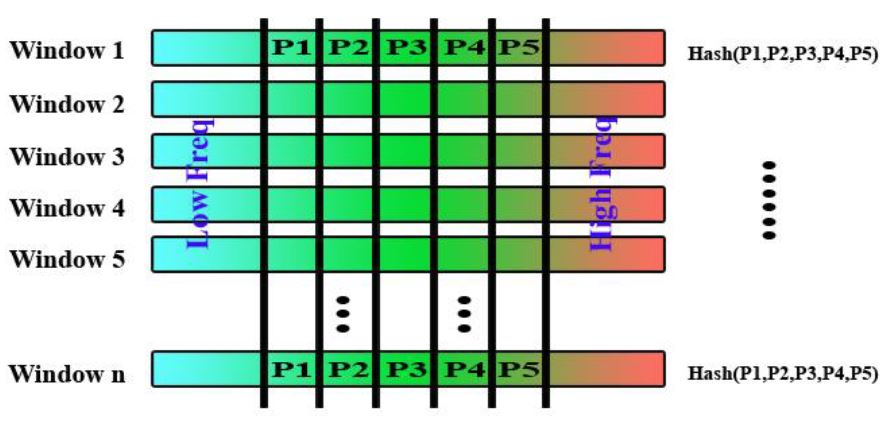
\includegraphics[scale=0.7]{HashGeneration}
    \caption{Extracting peaks and generating a hash value\cite{Nishan}}
    \label{fig:fingerprint}
\end{figure}

\vspace{12pt}

Timbre, tempo, timing, structure, key, harmonization and lyrics are the basic musical facets that can be 
identified\cite{SerraBook}.Timbre, also known as tone colour is the music facet which makes a difference of different 
sound productions even when they have the same pitch and loudness. Simply it is what makes a difference between a piano 
and a violin playing the same note at the same volume. Timbre can be changed due to the use of different sound enhancing 
and processing techniques or to the use of different instruments and configurations. Tempo is the speed or pace of the 
music which can be easily changed by playing the music in different speeds. The music facet of timing is rhythmic structure 
of the music which can be altered by the changes to the drum section. Structure is the arrangement of music sections, and
music structure alterations can be made while remastering. Key, harmonization and lyrics are 
tonality, chords and words of the music which can be altered while remastering.
\vspace{12pt}

In order to identify remastered music in radio broadcasts,
existing literature on cover song identification and music similarity measures can be used as foundation study to this 
research. Directly implementing a cover song identification method or a music similarity measure to identify remastered 
music in radio broadcasts is not possible as there is limited time to do the identification and it is not just 
comparing two music clips to find similarity, but comparing a radio broadcast with more than twenty thousand song database.